\documentclass[letterpaper, 10 pt, onecolumn]{ieeeconf}  

\IEEEoverridecommandlockouts                              % This command is only
                                                          % needed if you want to
                                                          % use the \thanks command


\usepackage{graphicx}
\usepackage{amsmath}
\usepackage{amssymb}
\usepackage{hyperref}

\title{\LARGE \bf Machine Learning Project Proposal: Solar Flare Forecasting}

\author{Dave Achyut$^{1}$ and J. Marcus Hughes$^{1}$ and Mahesh Parab$^{1}$% <-this % stops a space
\thanks{$^{1}$Department of Computer Science, University of Colorado Boulder, Boulder, CO}%
}

\begin{document}
\maketitle
\thispagestyle{empty}
\pagestyle{empty}

%%%%%%%%%%%%%%%%%%%%%%%%%%%%%%%%%%%%%%%%%%%%%%%%%%%%%%%%%%%%%%%%%%%%%%%%%%%%%%%%
\begin{abstract}
Solar flares can impact humans in many negative ways such as disrupting communications, harming astronauts, damaging electrical power grids. Our project will focus on forecasting the future brightness once one has begun. 

\end{abstract}

%%%%%%%%%%%%%%%%%%%%%%%%%%%%%%%%%%%%%%%%%%%%%%%%%%%%%%%%%%%%%%%%%%%%%%%%%%%%%%%%
\section{MOTIVATION AND BACKGROUND}
Solar flares are sudden releases of energy from the Sun with harmful effects such as disrupting electrical power grids, damaging satellites, and endangering astronauts. Many groups are working to forecast whether this will be a solar flare hours to days in the future \cite{nishizuka}. That problem is very challenging. A smaller, interesting problem that is not well explored is predicting a flare's evolution on a shorter time scale of minutes to hours. During a flare, the observed brightness increases rapidly and then decreases as the flaring event ends as shown in Figure \ref{fig:example}. Our task is to forecast how bright a flare will be in the future after observing a portion of it in a given wavelength interval (referred to from here on as a passband). Predicting when and how bright a flare will peak will allow quicker response for space weather forecast centers and ultimately quicker alerts. Even more so, there are scientific questions that can be addressed by knowing how well we can predict (the stability of flaring regions), what information is most useful in prediction (insight on what the most important drivers in flaring are), and when the regressor fails (understanding of potentially different types of flares).

\begin{figure}[h!]
    \centering
    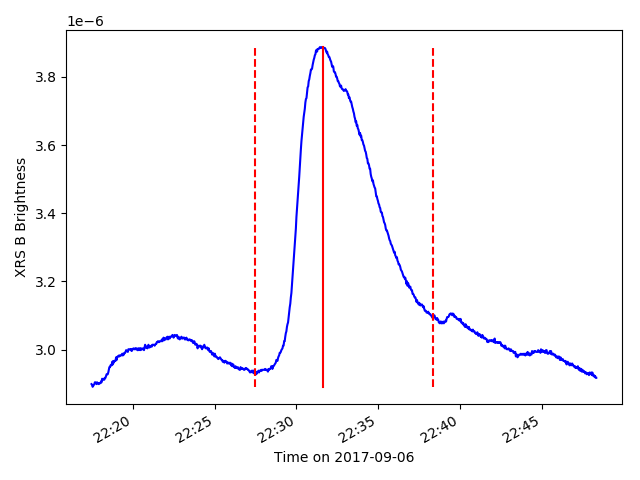
\includegraphics[scale=0.75]{flare_example.png}
    \caption{This bright flare from September 6th, 2017 shows the X-ray brightness change. The first dotted, vertical, red line indicates where the flare begins. The solid, vertical, red line indicates the peak of the flare. The final dotted, vertical, red line indicates the time the flare ends. We would like to forecast the brightness of the flare in real time, thus being able to estimate when and how bright it will peak and how when it will end and return to the brightness before the event.} 
    \label{fig:example}
\end{figure}

\section{PROBLEM STATEMENT}

For a given flare, we will chunk the flare observations into smaller time intervals, represented by $k$-dimensional vectors $\vec{x}^i = [x_{i,1} \hdots x_{i, k}]$. From these observations, we train a regressor that predicts $[x_{i,k+1} \hdots x_{i, k+M}$. 

\section{DATA SOURCES}
Our primary event list is the \textit{Geostationary Operational Environmental Satellite} (GOES) flare catalog. We have written a Python script to retrieve this database using the SunPy API and have 90,701 flares between 1975 and 2018 \cite{sunpy}. Our main data are the GOES X-ray Sensor (XRS) observations of the Sun. Roughly every 3 seconds, GOES-XRS reports the brightness of the Sun in two passbands: a short wavelength passband from 0.5 to 4 angstroms called the A passband and a long wavelength passband from 1 to 8 angstroms called the B passband. D. We have written Python scripts that will retrieve this data using the SunPy API \cite{sunpy}. Since the median flare duration is 840 seconds we have 280 GOES-XRS observations for each flare in each passband. Each flare can be divided into multiple sections of a set observation window, $k$, i.e. from observing $k$ datapoints we forecast the future. As discussed below, we will vary $k$ to determine an optimal length maximizing the trade-off between instantaneous predictions from only a few observations and accurate observations after observing most of a flare's lifetime. Thus, every moment in the flare can be associated with an observational history and future meaning our dataset is greater than 24 million data points. 

This event list is curated by hand and may miss some flares. We have obtained a larger flare list, the \textit{Reuven Ramaty High Energy Solar Spectroscopic Imager} (RHESSI) flare list that has 121,180 flares between 2002 and 2018. We can use this to augment the GOES list if we find we need more events. However, the list appears to include erroneous events. Similarly, we have obtained the flare list from Ryan et al. (2016) that identifies even more events and discriminates ``complex" flare events when an event has multiple flares in rapid succession before returning to normal brightness \cite{ryan}. This list has 173,988 flares from 2010 to 2018. 

In addition to augmenting the event list, we can augment the feature list for each flare since knowing information about the state of the Sun beyond merely the historical brightness of the Sun would be helpful. Upon talking with domain experts, we have identified a list of potentially helpful datasets that we have developed an API to fetch from various sources:
\begin{itemize}
    \item \textbf{\textit{Solar Dynamics Observatory} (SDO) Helioseismic and Magnetic Imager (HMI) magnetograms}: Flares are driven by the magentif fields of the Sun. When the magnetic fields become complex with positive and negative polarities mixing, there is greater potential for flares. Magnetograms are images that directly allow us to estimate this mixing. We are considering using these images in some convolutional neural network interface to extract features or manually extracting features, e.g. the standard deviation of the mixing around the flaring region. 
    \item \textbf{\textit{Spaceweather HMI Active Region Patch (SHARP)}}: Another way to use the HMI images is to fetch the SHARP entry for the active region, active regions are regions on the Sun that are bright in EUV and have especially strong magnetic fields, that the flare belongs to. Unfortunately, our event list does not always denote the active region a flare belongs to, so we will either have to experiment with this feature on a subset of them or estimate which active region patch works best. 
    \item \textbf{\textit{Solar Radio Flux at 10.7 cm}}: The solar radio flux at 10.7 is regarded as a proxy for solar activity. We have developed a Python tool that can retrieve it from the University of Colorado's Laboratory for Atmospheric and Space Physics (LASP) online archive, the LASP Interactive Solar Irradiance Datacenter. This data could be beneficial in relating the current solar activity to flaring capability and linking similar flares in the Sun's 11 year activity cycle. 
    \item \textbf{SDO Atmospheric Imaging Assembly (AIA) extreme ultraviolet (EUV) images}: Ultraviolet images reveal high-energy, complex structures on the Sun. By looking at EUV images we can also identify where filaments and other solar structures that can impact the flaring capability are. Similarly, we can refer to the Heliophysics Event Knowledgebase which provides segmentation masks for the Sun and these events. (However, these are not always reliable.) 
    \item \textbf{Large Yield Radiometer (LYRA) and Extreme Ultraviolet Variability Experiment (EVE) }: LYRA and EVE \cite{lyra} are EUV sensors that output light curves, scalar values over time, of various solar measurements. These may be helpful and have similar data to AIA's images, just in a one-dimensional time series. 
\end{itemize}

Depending on how we choose to use these lists and features, we will have dozens to hundreds of features for each of our 23+ million flare sections, corresponding to 120,000+ flares. Every flare section has ground truth data we can use. We will keep a hold-out set of flares 

\section{INTERESTING SUB-PROBLEMS AND QUESTIONS}
There are many related questions that we will explore as time allows through our approaches and experiments:
\begin{itemize}
\item Are there different types of flares? In operational solar weather forecasting, flares are classified based on their peak X-ray intensity. However, this ignores all spatial structure and how they evolve. We may be able to use our database for unsupervised clustering to identify kinds of flares from a data science perspective. If we can identify these types without using the full flare observation, we may be able to add it as a feature to augment our forecast performance. Regardless of our utility, it is of scientific interest. 
\item Given X-ray observations, can we predict the EUV light curve? They are inherently related by the physics of the Sun, but the relationship can become complicated. There may be scientific conclusions if only some "types" of flares can be mapped this way. 
\item What features optimize our prediction performance? How far into the future can we reliably forecast? Conversely, what features are least important and how does that compare to the physics intuition of importance?
\end{itemize}

\section{PROPOSED APPROACHES}
We will try the following learning techniques and compare their results:
\begin{enumerate}
    \item \textbf{Baseline model} - Given $k$ observations $X = [x_i, \hdots , x_{i+k}]$, we assume that the next $m$ observations is the mean of $X$. This model has high bias, and is expected to perform poorly on the test set.
    \item \textbf{Linear Regression} - We will fit a linear model to the training data. We will train the data with and without regularization and compare their accuracy on the test set. Typically, the mean square error is used as an error measure. However, since the absolute error values can vary with the intensity of the flare, we can used a more scale-dependent approach like the Mean Absolute Percentage Error (MAPE). We will also explore the effect of feature selection on the test accuracy.
    \item \textbf{Random Forest} - We will fit a Random Forest regressor to the data. Each tree in the forest will find the locally optimal feature to split the data by minimizing an impurity measure like MAPE. Feature importance can be calculated as the decrease in node impurity weighted by the probability of reaching that node. Also, we will explore the effect of limiting tree depth on the test accuracy.
    \item \textbf{Long short-term memory (LSTM)} - LSTMs are a deep learning technique well-suited to time series data, as they can efficiently remember important events in the data that influence future predictions. However, this approach will not provide any insight into feature importance, so we will implement feature selection to observe its effect on the model accuracy.
\end{enumerate}

\section{PROPOSED TIMELINE AND WORK DIVISION}
\begin{itemize}
    \item \textbf{November 1:} Submit proposal
    \item \textbf{December 7:} Completed paper written for final revision
    \item \textbf{December 14:} Submit project write-up by 5pm 
    \item \textbf{December 15:} Prepare poster 
    \item \textbf{December 17:} Present poster describing project
\end{itemize}

\begin{thebibliography}{99}
\bibitem{sunpy} Hughitt et al., 2012, SunPy: Open Source Solar Data Analysis Tools for Python at \url{sunpy.org}
\bibitem{lyra} M. Dominque et al., 2013, \textit{Solar Physics}, 286, 1, 21-42 
\bibitem{nishizuka} N. Nishizuka et al., 2018, \textit{The Astrophysical Journal}, 858, 113
\bibitem{ryan} D.F. Ryan, D. F. Ryan,  M. Dominique, D. Seaton, K. Stegen and A. White, 2016, \textit{Astronomy and Astrophysics}, 592, A133
\end{thebibliography}

\end{document}
